\documentclass[compress]{beamer}

\usepackage[utf8]{inputenc}
\usepackage{graphicx}
\usepackage{varwidth}
\usepackage{beamerthemesplit} 

\usepackage[english]{babel}
\usepackage[backend=bibtex]{biblatex}
\addbibresource{bibliography.bib}

\useoutertheme{miniframes}


\usetheme[progressbar=frametitle]{Madrid}
\usefonttheme{professionalfonts}
\setbeamertemplate{itemize items}[triangle]
\setbeamertemplate{enumerate items}[default]
\usecolortheme{beaver}

%Information to be included in the title page:

\title[Exoplanets survey via SL techniques]{A bird’s-eye view on the habitability of exoplanets via statistical learning techniques}

\author{Marzio De Corato}

\subtitle{Project for the exam: Machine learning, statistical
learning, deep learning and artificial intelligence - Unsupervised Learning}

\begin{document}

\frame{\titlepage}

\section{Intro}

\begin{frame}
\frametitle{Overview}
\begin{itemize}
\item\textbf{FINAL GOAL}: Survey the performances of different statistical learning algorithm in the prediction of exoplanets habitability
\item\textbf{DATASET}: Planetary Habitability Laboratory @ UPR Arecibo \cite{exoplanets-catalog}
\item\textbf{ALGORITHMS}: Decision Tree, Random Forest, Support Vector Classifier, Logistic Regression, Linear and Quadratic Classifier
\end{itemize}
\end{frame}

\section{Data}

\begin{frame}
\frametitle{Exoplanets habitability - theoretical background}
\begin{columns}
\column{0.5\textwidth}
\begin{itemize}

\item\textbf{HABITABILITY}: Rocky planets where water is present in liquid phase 
\item\textbf{LIQUID PHASE OF WATER}: At first order, if water is present, the liquid phase is controlled by the surface temperature 
\item\textbf{ATMOSPHERE}: The atmosphere (CO$_{2}$) influences the surface temperature trough the greenhouse effect
\item\textbf{H$_{2}$ and CH$_{4}$}: Other gases such as H$_{2}$ and CH$_{4}$ can produce the greenhouse effect, thus the habitable zone can be extended 
\end{itemize}
\column{0.4\textwidth}
\begin{minipage}{\textwidth}
  \centering
  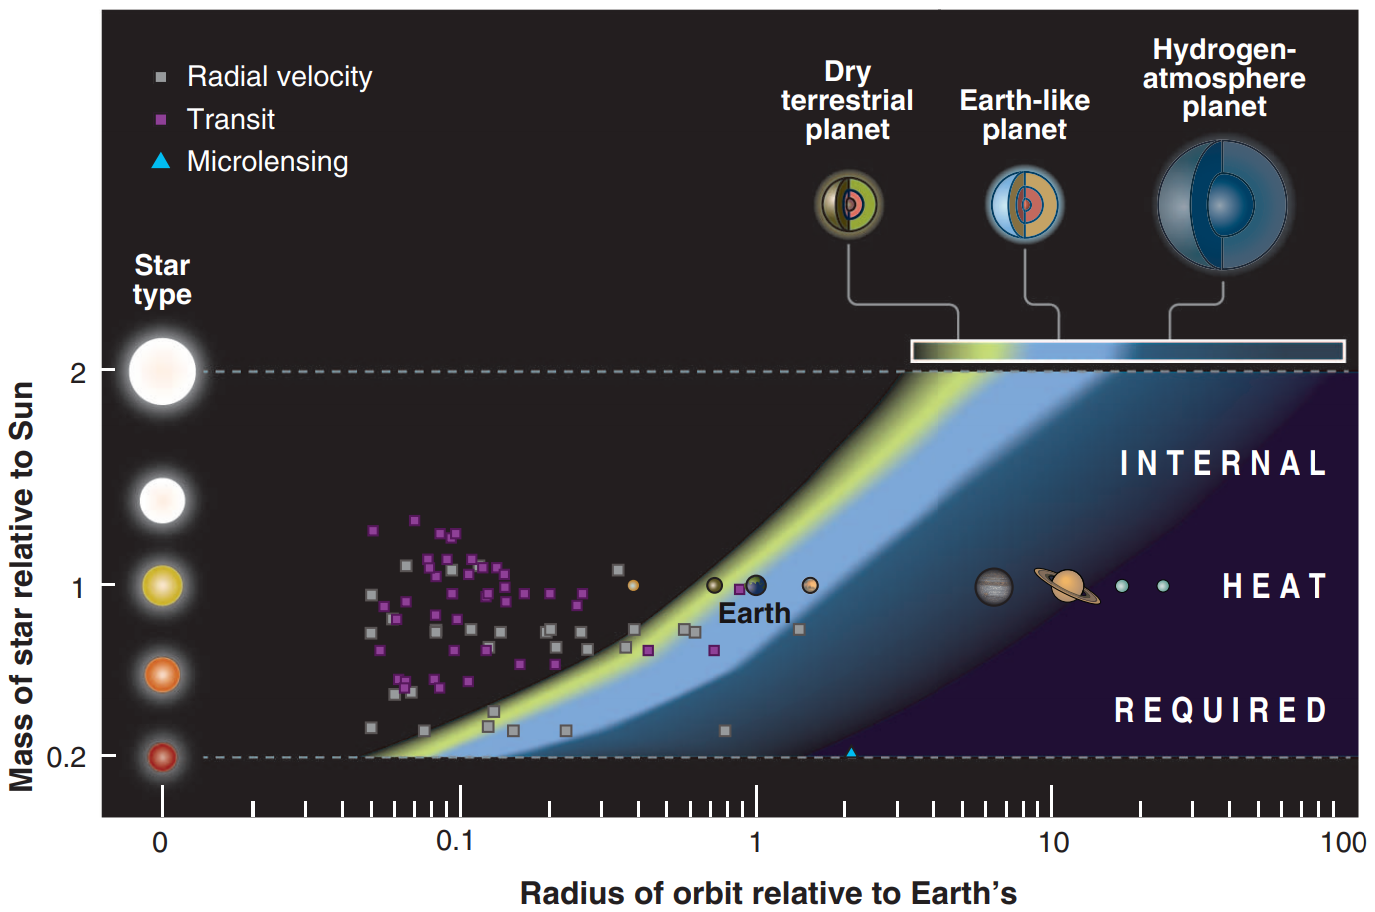
\includegraphics[width=\linewidth,]{Pic/Planets_habitability_Seager.png}
\end{minipage}%

\end{columns}
\end{frame}





\begin{frame}[t,allowframebreaks]
\frametitle{References}
\printbibliography
\end{frame}

\end{document}